\documentclass{article}
\title{ECE 311 -- Homework 2}
\usepackage[margin=1in]{geometry}
\usepackage{graphicx}
\usepackage{pdfpages}
\usepackage{fancyhdr}
\usepackage{enumitem}
\usepackage{pdfpages}
\usepackage{amsmath}
\usepackage{amssymb}
\usepackage{float}
\pagestyle{fancy}
\fancyhf{}
\fancyhead[L]{Gianni Avilan-Losee}
\fancyhead[C]{ECE 311}
\fancyhead[R]{Homework 2}
\fancyfoot[C]{\thepage}
\usepackage{microtype}
\usepackage{textcomp, gensymb}
\author{Gianni Avilan-Losee}
\setcounter{section}{1}
\begin{document}

\includepdf[pages=-]{homework-2_cover-page.pdf}
\begin{enumerate}[label=\thesubsection]
	\setcounter{section}{8}
	\setcounter{subsection}{1}
	\item
		\textbf{Note}: the following assumes that, unless otherwise notated, voltages and current magnitudes are given in rms values. Additionally, when calculating voltage, current, and impedance in \textit{phasor} form, \(\overline{V}_{an}\) is used as the reference voltage; that is, it is assumed to have a phase angle \(\theta = 0\degree\). Finally, I have assumed throughout this problem that the wye-connected source is powering a delta-connected load.
	\begin{enumerate}[label=\alph*)]
			\item
			For a sinusoidal voltage in a three-phase system given in the form \(V_\mathrm{{max}}\sin{(\omega t \pm \theta)}\), the rms phase voltage \({V}_{ph}\) is given by \[
				{V}_{ph} = \frac{V_{\mathrm{max}}}{\sqrt{2}} = \frac{340}{\sqrt{2}} = 240.42 \ \mathrm{V}.
			\] 
		\item The line-to-line rms voltage in a three-phase, balanced, wye-connected source may be found using the phase voltages, where 
		\begin{align*}
			{\overline{V}_{an}} = V_{ph}\angle{0\degree} \\
			{\overline{V}_{bn}} = V_{ph}\angle{-120\degree} \\
			{\overline{V}_{cn}} = V_{ph}\angle{120\degree},
		\end{align*}
		and 
			\begin{align*}
			&\overline{V}_{ab} = \sqrt{3}V_{ph}\angle{30\degree} \\
			&\overline{V}_{bc} = \sqrt{3}V_{ph}\angle{-90\degree} \\
			&\overline{V}_{ca} = \sqrt{3}V_{ph}\angle{150\degree}.
			\end{align*}
			Therefore, solving just for the rms value of the line-to-line voltages, \[ 
			V_{ab} = V_{bc} = V_{ca} = \sqrt{3}V_{ph} = 416.413 \ \mathrm{V}. 
		\]
	  \item The rms source current through a three-phase, wye-connected, balanced source, \(I_{a}\) may be found as \[
				\frac{I_{\mathrm{max}}}{\sqrt{2}} = \frac{100}{\sqrt{6}} = 70.711 \ \mathrm{A}
	  \]
		\item The rms value of the line current for any phase connected to a three-phase balanced load are found using a similar formula to phase voltage, \[
				I_a = I_b = I_c = \frac{I_{max}}{\sqrt{2}} = \frac{100}{\sqrt{2}} = 70.711 \ \mathrm{A}.
		\]
	\item The source's angular frequency in a three-phase balanced system is the same in all three lines, given in the time-dependent formula for voltage and current as \(\omega\), in radians per second. Converting \(\omega = 377 \frac{\mathrm{rad}}{\mathrm{s}}\)to units of frequency \(f\) in hertz, \[
			f = \frac{\omega}{2\pi} = \frac{377}{2\pi} = 60 \ \mathrm{Hz}.
	  \]  
	\item Power factor may be found as the cosine of the phase angle difference between voltage and current, \(\theta_{VI} = \theta_{V} - \theta_{I}\), \[
			P.F. = \cos{(\theta_{VI})} = \cos{(-0.3491)} = 0.9397 \ \mathrm{(leading)},
	  \] 
		since the phase angle difference \(\theta_{VI}\) is negative, implying a capacitive load and a leading current waveform.
	\item Three-phase real power \(P = 3P_{ph} = 3V_{ph}I_{ph}\cos{(\theta_{VI})}\), so \[
			P = (3 \times 240.416 \times 70.711)\cos{(-0.3491)} = 47.924 \ \mathrm{kW}. 
	  \]
	  \item Three-phase reactive power \(Q = 3P_{ph}\cos{(\theta_{IV})},\) so \[
				Q = (3 \times 240.416 \times 70.711)\sin{(-0.3491)} = -17.445 \ \mathrm{kVAr}. 
	  \] 
	\item Given a delta-connected three-phase balanced load, the load impedance \(\overline{Z}\) may be found using
		\[
			\overline{Z} = \frac{\overline{V}_{ab}}{\overline{I}_{ab}} = \frac{\overline{V}_{bc}}{\overline{I}_{bc}} = \frac{\overline{V}_{ca}}{\overline{I}_{ca}}.
		\]
		Finding \(\overline{I}_{ab}\), we may use the relationship
		\[
			\overline{I}_{a} = \sqrt{3} \ \overline{I}_{ab}\angle{-30\degree} \Rightarrow \overline{I}_{ab} = \frac{70.11}{\sqrt{3}}\angle{50\degree} = 40.83\angle{50\degree} \ \mathrm{A}.
		\]
		Then, \[
			\overline{Z} = \frac{416.41 \angle{30\degree}}{40.83\angle{50\degree}} = 10.20 \angle{-20\degree} \ \ohm.
		\]
	\end{enumerate}
	\setcounter{subsection}{2}
	\item
		\begin{enumerate}[label=\alph*)]
			\item \(\overline{V}_{an}\) may be found as \[
					\overline{V}_{an} = V_{ph}\angle{0\degree}.
			\]
			Thus, finding \(\overline{V}_{an}\), \[
				\sqrt{3}V_{ph}\angle{150\degree} = \overline{V}_{ca} \Rightarrow \overline{V}_{an} = \frac{480\angle{-60\degree}}{\sqrt{3}\angle{150\degree}} = 277.13\angle{150\degree} \ \mathrm{V}. 
			\] 
		  \item \(\overline{I}_a\) may be found as \[
				\overline{I}_a = {I}_b\angle{(\theta_{I_b} + 120\degree)} = 20\angle{-120\degree} \ \mathrm{A}.
		  \] 
			\item The phase angle difference \(\theta_{VI} = -90\degree\), so \[
					P.F. = \cos{(-1.5708)} = 0 \ \mathrm{(leading)},
			\]
			implying a purely capacitive load.
			\item Real power \(P\) may be found as \[
					P = 3P_{ph}\cos{(\theta_{VI})} = (3 \times 277.128 \times 20)\cos{(-90\degree)} = 0 \ \mathrm{W}.
			\]
		\end{enumerate}
		\setcounter{subsection}{5}
		\item
		\begin{enumerate}[label=\alph*)]
			\item Using \(\overline{V}_{ab}\) as the reference voltage, with a phase angle of \(\theta=0\degree\), we may find the voltage across the load as \[
					\overline{V}_{an} = \frac{V_{ab}}{\sqrt{3}}\angle{-30\degree} = 99.88\angle{-30\degree} \ \mathrm{V}, 
			\] 
			and the transmission line current as \[
				\overline{I}_{a} = \frac{\overline{V}_{an}}{Z} = \frac{99.88\angle{-30\degree}}{5\angle{36.87\degree}} = 19.98 \angle{-66.87\degree} \ \ohm
			\]
		  \item Given a phase angle difference \(\theta_{VI} = 66.87\degree\),
			\begin{align*}
				&P.F. = \cos{(1.1671)} = 0.3928 \ \mathrm{(lagging)}, \\
				&S = P + jQ = 3V_{an}I_{a} = 3 \times 99.88 \times 19.98 = 5.987 \ \mathrm{kVA}, \\
				&P = S\cos{(\theta_{VI})} = [5.987 \times 10^3] \cos{(1.202)} = 2.352 \ \mathrm{kW}, \\
				&Q = S\sin{(\theta_{VI})} = [5.987 \times 10^3]\sin{(1.202)} = 5.506 \ \mathrm{kVAr}.
		  \end{align*} 
		  \item The following diagram was generated in MATLAB:
				\begin{figure}[H]
				  \centering
				  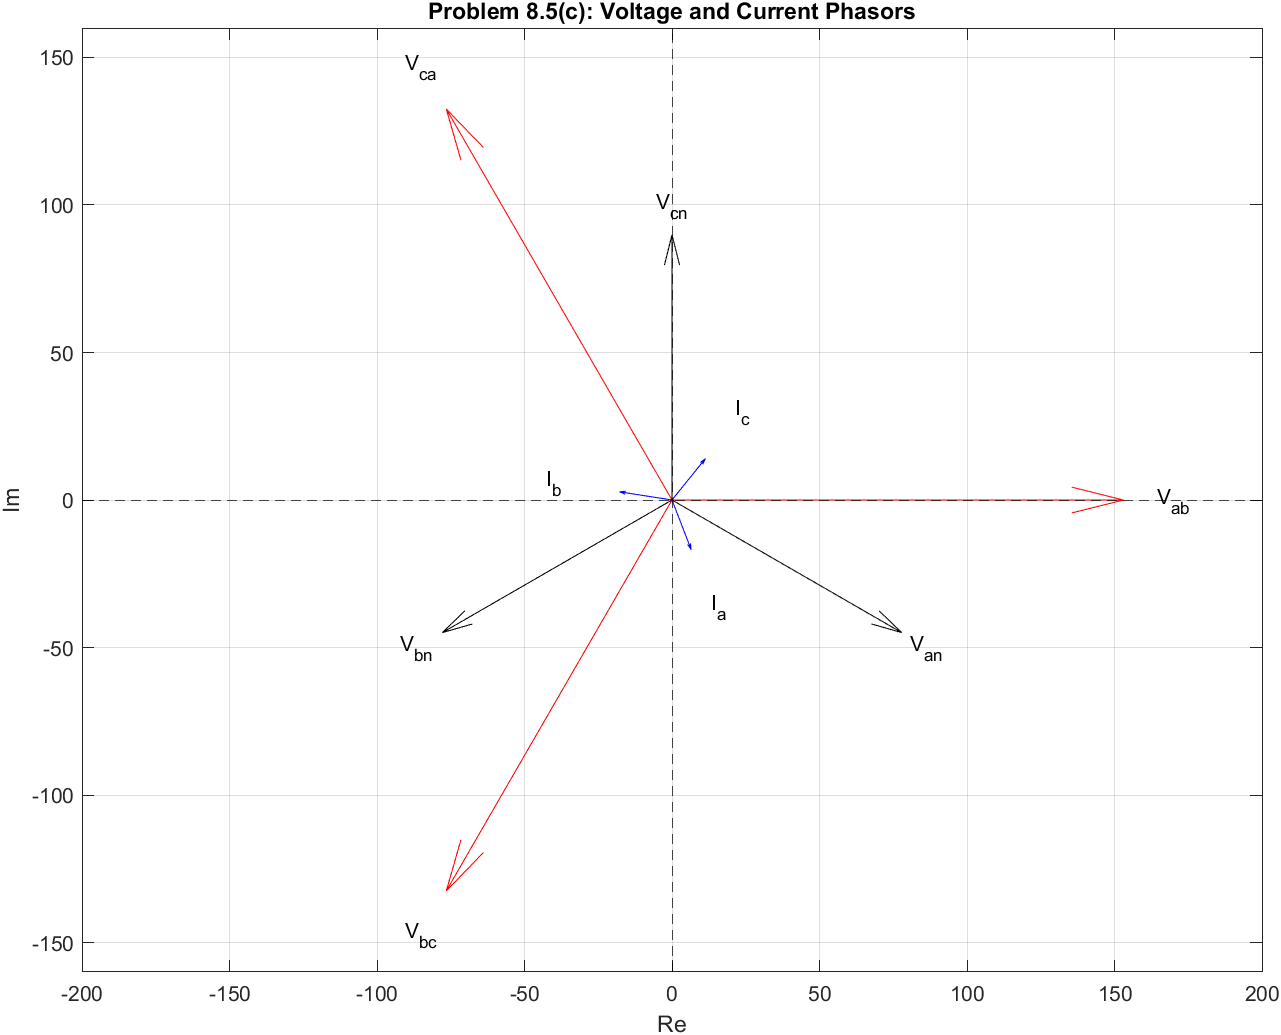
\includegraphics[width=0.8\textwidth]{homework-2_fig-1.png}
				  \caption{Voltage and Current Phasors}
				  \label{fig:V_I_ph}
				\end{figure}
		\end{enumerate}
		\setcounter{subsection}{6}
		\item
			\begin{enumerate}[label=\alph*)]
				\item The total current through one phase A of the transmission line can be derived using KCL, and simply adding the current through the parallel loads together, \[
						\overline{I}_{a} = 20\angle{25.84\degree} + 30\angle{-36.87\degree} = 43.01\angle{-12.46\degree} \ \mathrm{A}. 
				\] 
				Then, the other two phases can be derived by simply shifting their phase angles \(120\degree\) backwards, \begin{align*}
					&\overline{I}_a = 43.01 \angle{-12.46\degree} \ \mathrm{A} \\
					&\overline{I}_b = 43.01 \angle{-132.46\degree} \ \mathrm{A} \\
					&\overline{I}_c = 43.01 \angle{107.54\degree} \ \mathrm{A}. 
				\end{align*} 
				\item Assuming a reference voltage phase angle of \(\theta = 0\degree\) for \(V_{an}\), we may derive the power factor as \[
					P.F. = \cos{(\theta_{VI})} = \cos{(0.2175)} = 0.9764 \ \mathrm{(lagging)}.
		  \]
			\item Using the phase voltage \(V_{ph} = \frac{400}{\sqrt{3}} = 230.94 \ \mathrm{V}\), we may find real power as \[
					P = [3 \times 230.94 \times 43.01]\cos{(0.2175)} = 29.096 \ \mathrm{kW}.
			\]
	\end{enumerate}
	\setcounter{subsection}{11}
\item Given \(\overline{V}_{bn} = 120\angle{0\degree} \ \mathrm{V}\), \(\overline{V}_{an} = 120 \angle{120\degree} \ \mathrm{V}\), and \(\overline{V}_{ab} = 207.85\angle{150\degree} \ \mathrm{V}\). Then, \[
		\overline{I}_{ab} = \frac{\overline{V}_{ab}}{\overline{Z}} = \frac{207.85 \angle{150\degree}}{9\angle{30\degree}} = 23.09\angle{120\degree} \ \mathrm{A}. 
\]
  Converting load current to transmission line current, \[
		\overline{I}_{a} = \sqrt{3} \ \overline{I}_{ab} \angle{-30\degree} = \sqrt{3} \times 23.09\angle{90\degree} = 39.99 \angle{90\degree} \ \mathrm{A}.  
  \]
	Using the load current and voltage along with the phase angle difference to calculate real power consumed by the load, \[
		3I_{ab}V_{ab}\cos{(0.5236)} = 12.469 \ \mathrm{kW}.
	\]
\end{enumerate}
\end{document}
